\documentclass[11pt, a4paper]{article}
\usepackage{amsfonts, amsmath, hanging, hyperref, parskip, times}
\usepackage[numbers]{natbib}
\usepackage[pdftex]{graphicx}
\hypersetup{
  colorlinks,
  linkcolor=blue,
  urlcolor=blue,
  citecolor=blue
}

\let\section=\subsubsection
\newcommand{\pkg}[1]{{\normalfont\fontseries{b}\selectfont #1}} 
\let\proglang=\textit
\let\code=\texttt 
\renewcommand{\title}[1]{\begin{center}{\bf \LARGE #1}\end{center}}
\newcommand{\affiliations}{\footnotesize\centering}
\newcommand{\keywords}{\paragraph{Keywords:}}

\setlength{\topmargin}{-15mm}
\setlength{\oddsidemargin}{-2mm}
\setlength{\textwidth}{165mm}
\setlength{\textheight}{250mm}

\begin{document}
\pagestyle{empty}

\title{Interactive inspection of large data}

\begin{center}
  {\bf Edwin de Jonge$^{1^\star}$, Martijn Tennekes$^{1}$}
\end{center}

\begin{affiliations}
1. Statistics Netherlands\\[-2pt]
$^\star$Contact author: \href{mailto:e.dejonge@cbs.nl}{e.dejonge@cbs.nl}\\
\end{affiliations}

\keywords multivariate, visualization, large data, interactive

\vskip 0.8cm

We present \pkg{tabplotd3}, an interactive tool in \proglang{R} for inspecting large multivariate data consisting of millions of objects. 
\pkg{tabplotd3} allows to visually check for anomalies, patterns and missing values in bivariate relations in multivariate data, for categorical as well as numerical variables. The interface creates tableplots \citep{malik10} from very large \code{data.frame}s and allows to zoom in to individual observations. We applied the tool to the Dutch (virtual) census \citep{schulte}, creating a tableplot that depicts the 16.4 million inhabitants of the Netherlands. \\ 

  \begin{center}
    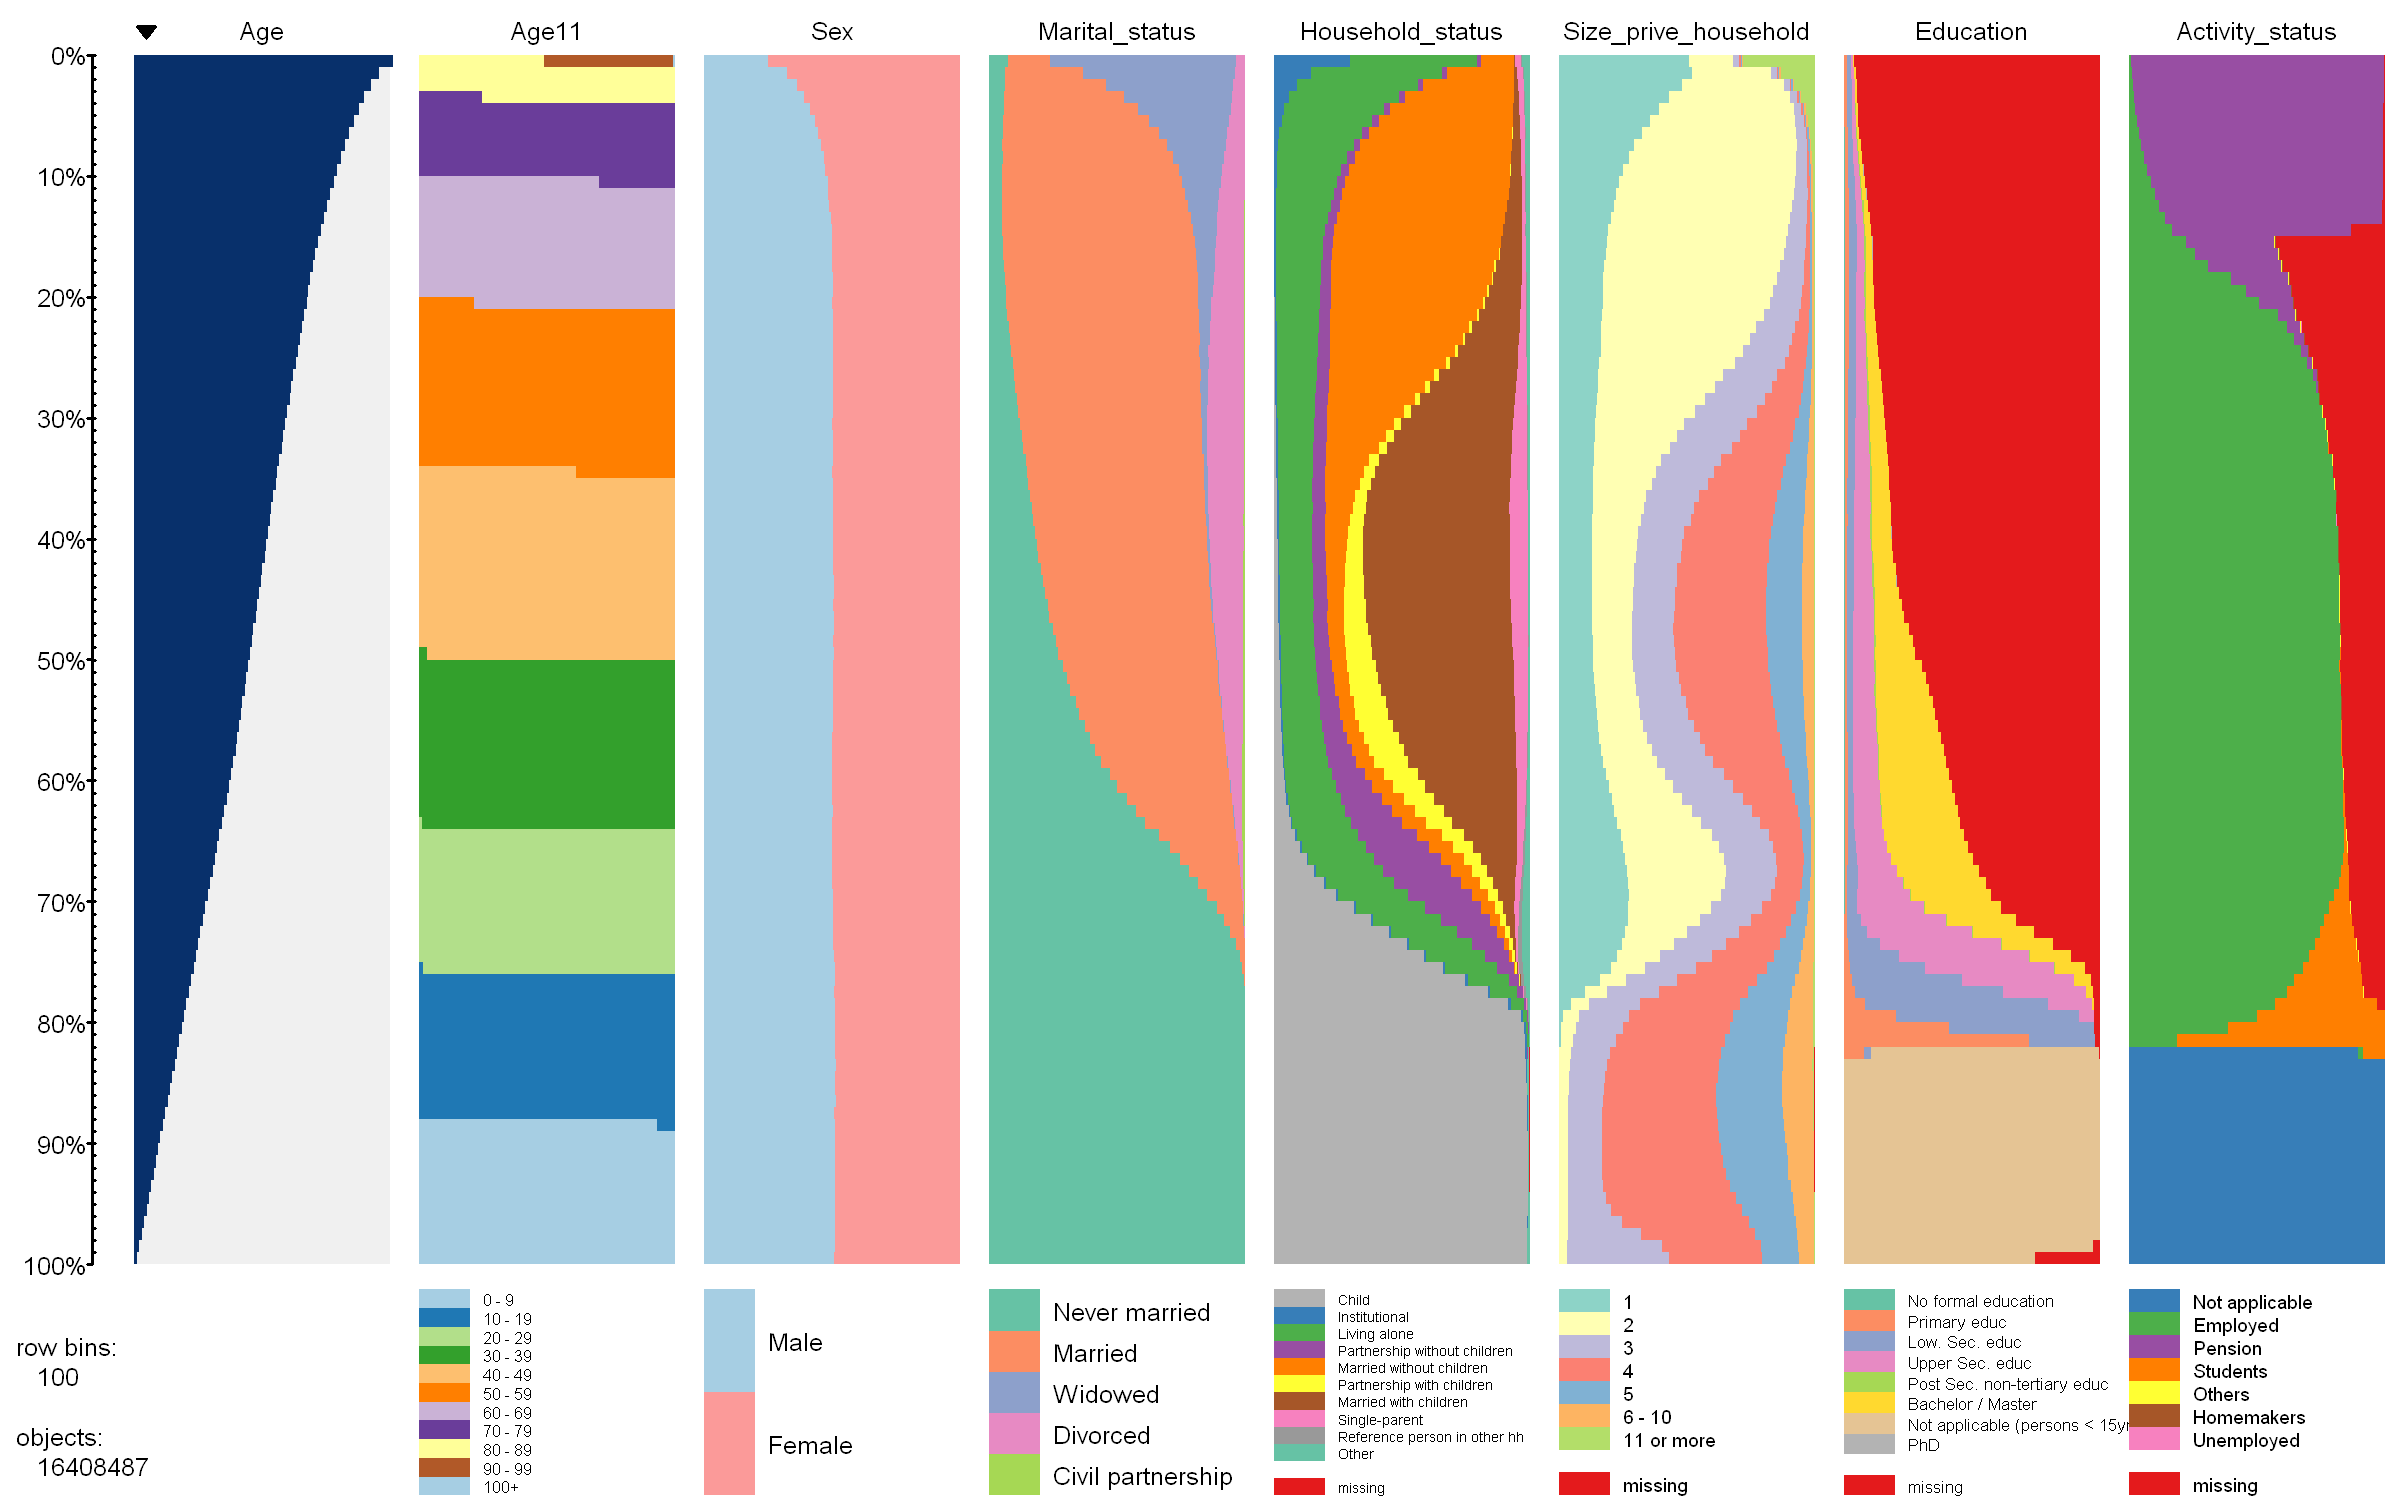
\includegraphics[scale=0.6]{VT2008}
  \end{center}
 
The presentation will describe tableplots, their use and implemention in \pkg{tabplot} and \pkg{tabplotd3}. The tool is an interactive web application. To allow interactive actions on very large \code{data.frame}s we implemented some aggregations methods in \proglang{C}. The user interface is in \proglang{javascript} and \proglang{SVG}. 
The tool builds on several other packages including \pkg{Rook}, \pkg{RJSONIO}, \pkg{ff}, and our non interactive \pkg{tabplot}. 

%% references: 
\bibliographystyle{chicago}
\bibliography{tabplotd3}

\end{document}
